\documentclass{article}
\usepackage[utf8]{inputenc}

\usepackage{geometry}
\geometry{
margin=30mm
}

\usepackage{tikz}
\usetikzlibrary{positioning}

\begin{document}

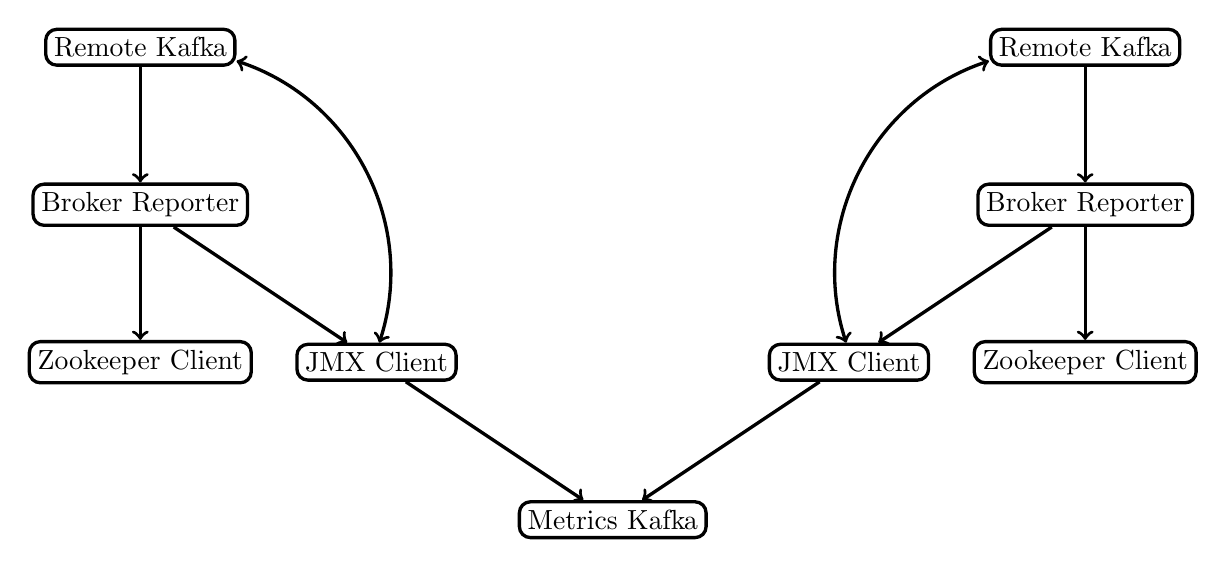
\begin{tikzpicture}[ % has a lot of options; consult the pgf manual
bend angle=45,
square/.style={rectangle, draw=black, fill=white, very thick, inner sep=3pt, minimum width=14mm},
rounded_square/.style={rectangle, rounded corners, draw=black, fill=white, very thick, inner sep=3pt, minimum width=14mm},
circle/.style={rectangle, rounded corners=2mm, draw=black, fill=white, very thick, minimum size=4mm},
both_arrow/.style={<->, very thick},
out_arrow/.style={->, very thick},
in_arrow/.style={<-, very thick},
above_edge_text/.style={above, midway, sloped}
]



\node[rounded_square](kafka_one) at (0,0) {Remote Kafka};
\node[rounded_square](kafka_two) at (12,0) {Remote Kafka};

\node[rounded_square](reporter_one) at (0,-2) {Broker Reporter};
\node[rounded_square](reporter_two) at (12,-2) {Broker Reporter};

\node[rounded_square](zookeeper_one) at (0,-4) {Zookeeper Client};
\node[rounded_square](jmx_one) at (3,-4) {JMX Client};
\node[rounded_square](jmx_two) at (9,-4) {JMX Client};
\node[rounded_square](zookeeper_two) at (12,-4) {Zookeeper Client};


\node[rounded_square](kafka_metrics) at (6,-6) {Metrics Kafka};



\draw[out_arrow](kafka_one) to [] node[auto,swap]{} (reporter_one);
\draw[out_arrow](kafka_two) to [] node[auto,swap]{} (reporter_two);

\draw[out_arrow](reporter_one) to [] node[auto,swap]{} (zookeeper_one);
\draw[out_arrow](reporter_one) to [] node[auto,swap]{} (jmx_one);
\draw[out_arrow](reporter_two) to [] node[auto,swap]{} (zookeeper_two);
\draw[out_arrow](reporter_two) to [] node[auto,swap]{} (jmx_two);

\draw[both_arrow](jmx_one) to [bend right] node[auto,swap]{} (kafka_one);
\draw[out_arrow](jmx_one) to [] node[auto,swap]{} (kafka_metrics);
\draw[both_arrow](jmx_two) to [bend left] node[auto,swap]{} (kafka_two);
\draw[out_arrow](jmx_two) to [] node[auto,swap]{} (kafka_metrics);

\end{tikzpicture}

\end{document}